\chapter{Implementation}

The execution of the projected features described earlier on is the focus of this section.
Functionalities are grouped by purpose and their details explained and discussed.
The navigation modes, content creation, content editing and review features are described.
To close this section, an alternative work flow is proposed for taking advantage of the Urban Sketcher features.


\section{Navigation}

Good navigation modes are paramount for the success of any 3D based system.
The nature of this system, with the availability of a large screen,
stroke-controlled input and the aim of allowing unexperienced users to take control
of the system quickly, made this requirement even more relevant.

According both to the task at hand and personal taste,
several alternative modes may be useful to users.
For tasks of simulating human movement, a \textbf{first person} based mode is expected.
When searching for scenario features and moving big distances, a \textbf{top-down view} manipulation mode can be of aid.
In occasions when an object is clearly the center of attention of the user,
such as shape exploration and modeling operations, a \textbf{view centered on the object} mode is helpful.
For giving an overview of the scenario and showcasing blocks of buildings, a \textbf{flight movement} mode might be interesting.

The first 3 of the 4 mentioned modes were implemented with regular menu/gate widgets.
The flight mode is multimodal, relying on arm tracking and speech controlled input.

\begin{figure}[ht]
	\centering
		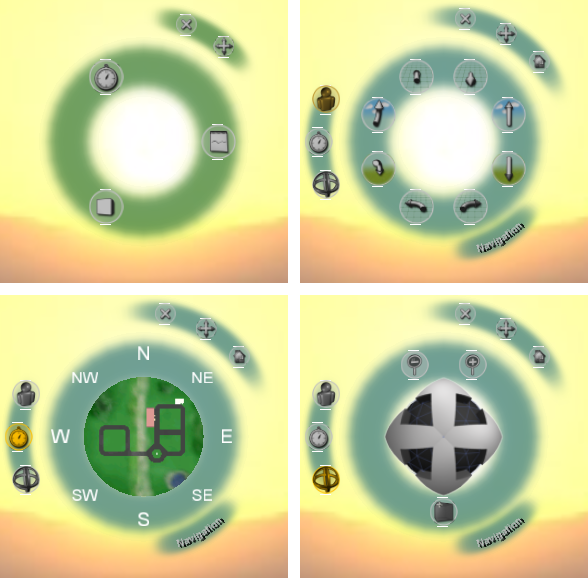
\includegraphics[scale=0.5]{gfx/main-nav-menus.png}
	\caption{Main menu and all 3 navigation menu modes}
	\label{fig:main-nav-menus}
\end{figure}


\subsection{First Person Mode}

This first person navigation mode (Fig.\ref{fig:main-nav-menus}, top right) is centered on the current point of view and works by triggering the displayed gates.
It maps an interface resembling most first person shooters, offering translations and rotations around the current point of view (POV).
It features 8 gates: 4 direction displacement gates and 4 rotation gates.
To stop the movement/rotation one can either trigger the gate again, effectively disabling the ongoing action
or by triggering a different gate action.
There are gates for moving forward/backwards, up/down, pitch up/down and yaw up/down
\footnote{The verbs pitch and yaw come from flight semantics: to pitch is to look up/downwards; to yaw is to turn relatively to the ground plane.}.

The choice for this mode's layout suffered several evolutions.
At early stages opposing directions where placed at opposite sides of the ring but this
made correction by triggering the opposite action difficult, so opposing actions are now close together.
In this mode a restriction of one enabled action at a time is imposed to keep the handling easy for novice users.

A helpful addition to this mode would be collision detection, to keep users from crossing walls and the ground.
This could also help users moving on ramps and staircases.
The application of SmartCam \cite{SMARTCAM}, commented on section \ref{SMARTCAM-LABEL} would also enhance this mode,
at least the physics spring model simulation part.



\subsection{Compass Mode}

A birds-eye-view of the POV is helpful in 3D exploration scenarions,
allowing the user to better perceive his positioning in the scenario.
The compass navigation mode (Fig.\ref{fig:main-nav-menus}, bottom left) was thought out for searching tasks.
It allows the user to move along the ground plane and turn around it.
The compass navigation mode has 2 distinct areas:
the center circle displays a top-down view of the scene centered on the user;
the outer ring displays the main compass directions.

The dragging gesture is increasingly more popular, and this mode uses it extensively:
dragging the center view translates the user along the ground plane;
dragging the outer ring rotates the POV, a concept easily grasped by test users.
The superimposed cardinal compass points are useful, particularly for people with a more technical background.

%In order for one to move, a dragging movement must be performed inside the top-down view.
%To reorient the user one must rotate the outer ring. The direction the user is facing can be read on the top part of the ring.

To enhance the reach of the translation movement, the Speed-dependent zooming \cite{SPEEDZOOM},
commented on section \ref{SPEEDZOOM-LABEL} could be applied,
translating drag velocity into exponential translation changes.

This mode could not be tested on multi-screen displays due to technical problems.
It was enthusiastically accepted on one-projector early tests.


\subsection{Examine Mode}

The examine mode is based on moving along the space close to the center of attention (Fig. \ref{fig:vsphere}).
It features 3 gates and a center sphere (see Fig.\ref{fig:main-nav-menus}, bottom right).

The user is offered a gate so a new center of attention can be set. This action is performed by
activating the gate and ending the same stroke at the desired center of attention.
Once this is done, a spherical widget allows performing rotations around the object by dragging the sphere.
Two additional gates allow zooming in and out to reveal more or less detail, respectively.

%The examine mode  allows the user to recenter attention on an object of the scene.
%It features 3 gates and a center sphere.
%The user must initially select the new center of attention by triggering the recenter gate,
%finishing the stroke at the desired object/location.
%Once the location is defined the remaining gates allow for zooming in and out the centered content
%while the sphere allows for repositioning the user on the space around the object -- 
%horizontal drags rotate horizontally, vertical moves vertically.

For the users who got the grip of this mode, it has revealed itself a very efficient way
for both looking around and repositioning oneself.
Only laser-tracking problems inhibited a better use of repeatedly re-centering operation for movement.


\begin{figure}[ht]
	\centering
		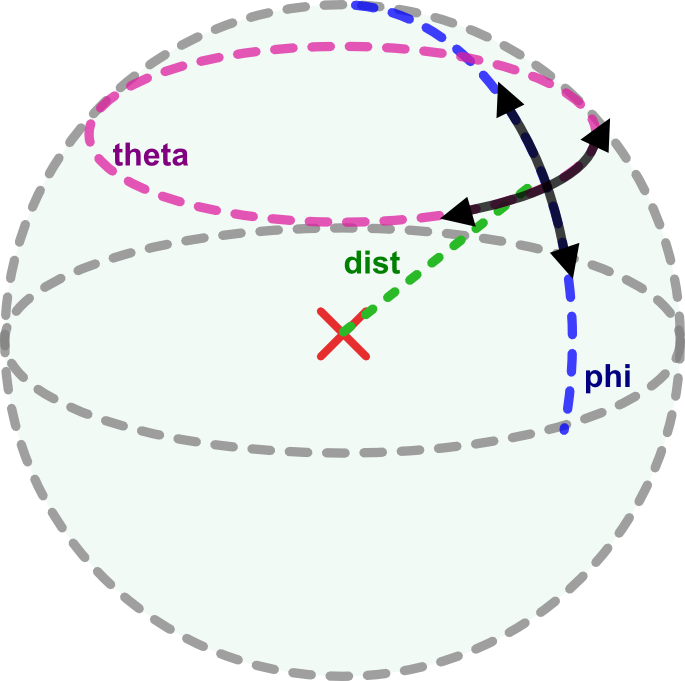
\includegraphics[scale=0.6]{gfx/virtual-sphere.png}
	\caption{Concept supporting examine mode}
	\label{fig:vsphere}
\end{figure}


\subsection{Multimodal Flight Mode}

This mode is the implementation of \ref{FLIGHT-DESIGN-LABEL} Arm Posing Flight Mode.
It is an alternative navigation mode. Since it affects the point of view, this task can't be performed by
several people simultaneously, therefore unlike most of the system this navigation mode has global states
-- the user might be either stationary of flying (see Fig.\ref{fig:flight}).

The user starts interacting by having his arms extended toward the screen.
In order to begin flying the command ``Begin flying'' must be given.
To stop at any time one only needs to say ``Stop flying''
\footnote{Although semantically inconsistent, the words begin and stop were used after performing speech recognition
tests with both start/stop, begin/end and begin/stop, concluding that this combination had the better recognition ratio.}.

Controlling flight speed works by measuring the distance between hands -- the closer they are to each other the faster
the flight speed is. If the arms do a wide enough angle between them the flight comes to an halt.
Changing the flight orientation relatively to the ground is achieved by setting the arms angle with the ground at opposing directions,
with a bigger difference between these angles generating a faster rotation movement. If the user wants to turn right, for instance,
he has to raise the left arm and lower the right one.

To change flight altitude both arms must be oriented in the same direction relatively to the ground plane
-- either both raised or lowered. Again, the higher the angle is from the original forward pose position
the bigger the flight altitude shift is.

\begin{figure}[ht]
	\centering
		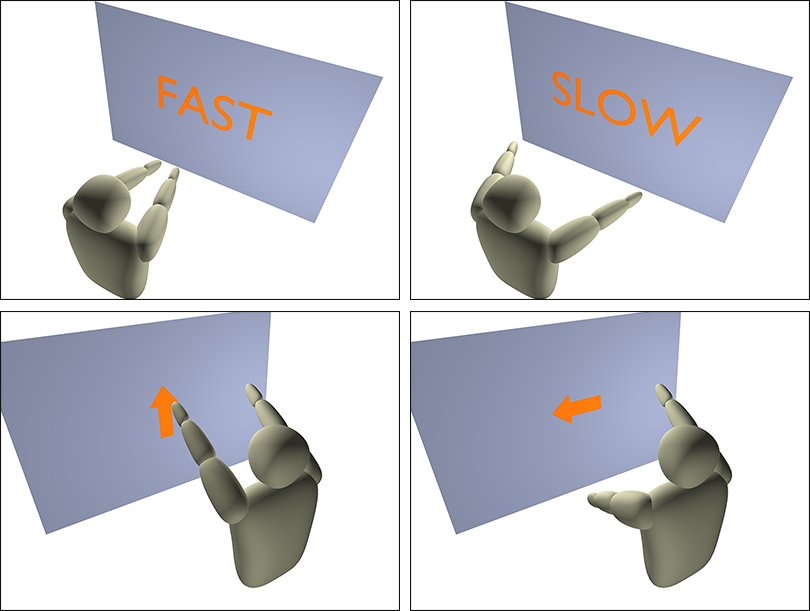
\includegraphics[scale=0.3]{gfx/flight.png}
	\caption{Flight mode: controlling speed and direction}
	\label{fig:flight}
\end{figure}


\subsection{Other navigational modes}

In addition to the navigation modes made available in the system, the following modes might be of use.

The multimodal ``go-to-here'' \TODO{REF}, with a combination of laser pointing to the destination
and speech command to trigger the movement. This mode was requested on the final tests.

The stroke-defined path, as suggested on the Path Drawing \cite{PATH3D}, discussed on section \ref{PATH3D-LABEL}.
It would be useful to experiment this mode, but the requirements for its application were unmatchable:
Igarashi's system uses a third person view with explicit avatar rendering. Moreover,
Urban Sketcher stroke-based interface makes it hard to map a movement path stroke
-- this would require multimodal integration with a ``move-like-this'' speech command.

During the navigation tests at Glasgow, users suggested the addition of a list of recorded locations.
The idea is for the user to get to an unrecorded and relevant point of view, such as a good fa�ade angle,
and trigger the record location action.
Recorded locations might be tagged by either speech recognition (example: ``record location \textbf{stadium front} now'')
or scribble text recognition. Later on resuming to the saved location would be a matter of invoking the related metadata.



\section{Content Creation}

The system's interface offers 3 families of shapes which can be instanced on the scene:
primitives, a set of previously generated shapes and set of known building styles from which to create buildings.
Primitives are the most versatile shapes since they support face and edge manipulation operations.
All shapes support simple transformations and cloning.

One uses building styles to create buildings on the scene. A library of generated shapes such as
people and trees serve as assets to populate the scene with details.
Primitives can be instanced as is or as building ground for custom shapes.

\begin{figure}[ht]
	\centering
		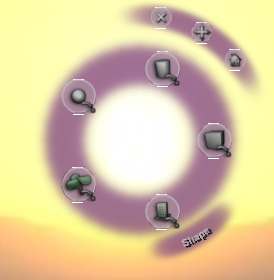
\includegraphics[scale=0.5]{gfx/shape.png}
	\caption{Shape menu}
	\label{fig:shape}
\end{figure}


\subsection{Shape Internal Structure}

A shape in this system is a boundary representation (B-REP) \cite{REP-SOLID}.
The shape surface is defined by two data structures:
an indexed array of \textbf{vertex positions}, used to store the position of each shape vertex;
an indexed array of \textbf{faces}, with every face being a counter-clockwise ordered set of 4 vertex indices.
An \textbf{edge} in the system is a pair of ordered vertex indices.
The ordering step makes the edge direction irrelevant for the edge definition, a desired feature.

Besides this information, each shape manages an auxiliary \textbf{edge map}.
This map associates a face to its bounding edges and vice versa.
The edge map allows efficient queries to be performed, such as:
\textit{which faces are bound by edge x};
\textit{what is the opposite edge of edge x in face y};
\textit{which other edges beside edge x make part of the face loop}.
These are all relevant queries for the implementation of internal shape operations.

Shapes offer methods to update their visual representation.
Shapes also make available a set of geometry modifying operations --
these are not only exposed to the user via UI, but also used by templates, as further explained.

In order to support undo operations, the memento design pattern \cite{DESPAT} was implemented.
A shape memento stores the internal structure of a shape at one point in time
and is able to restore that shape's state later on, if so requested.
A shape has a stack of mementos so multiple undo steps can be executed.


\subsection{Shape Instancing}

The instancing of shapes works using the Apply-to-Scene concept described on section \ref{design:apply-to-scene} Apply-to-Scene Creation
and the respective Figure \ref{fig:apply-to-scene}.
Every gate of this type has a small arrow running outwards as a hint to the user of this feature.
The user activates the gate of the desired shape and ends the stroke where he wants it to rest.


\subsection{Shape Templates}

A template is a shape recipe with input parameters, defining a way of obtaining the desired shape
by applying a set of operations, with the passed parameters affecting the final geometry.
Templates are not directly exposed on the system UI. They're currently used solely to generate building ceilings,
but could be extended for other means.

Templates make use of shape exposed operations to generate the final shape.
For instance, the creation of a 2-slanted ceiling starts from a regular box shape,
applying a sequence of 2 edge move operations.
\TODO{EXAMPLE 2-SLANTED CEILING}
Additional templates could be easily created to aid in the generation of repetitive structures
such as railings and staircases.


\subsection{Building Style}

A building is a complex shape, composed of side walls, a ceiling and a set of attached shapes enriching the fa�ades
with details such as doors, windows and balconies.

A building style is a set of rules and parameters, written according to an XML grammar. 
The system comes with a set of styles, with the user choosing the desired style to apply to the building he's about to create.
The building style factory is able to parse the style definition, instantiating and distributing attached shapes to make up
the fa�ades according to the chosen style.


\subsubsection{Building Style Structure}

The building style grammar defines building parameters such as
\textbf{floor-height}, \textbf{ceiling} parameters and \textbf{color-interval}s for the walls and ceiling.
It also defines a set of rules for the generation of the facade attachments that make up the final facades,
defined by the optional \textbf{front-facade} and the \textbf{facades} elements.

One can define the layout of a floor with the \textbf{layout} element, composed of 4 sections:
\textbf{left}, \textbf{center}, \textbf{right} and \textbf{other}.
Of these only the \textbf{other} section is required and the layout works by trying to fill the facade space with \textbf{center}, \textbf{left} and \textbf{right}s' contents if those are present, repeating \textbf{other}'s contents for filling the remaining space.

Inside these sections one can put any of the \textbf{us-element}s: \textbf{atom}, \textbf{group}, \textbf{sequence} and \textbf{random}.
An \textbf{atom} is the simplest \textbf{us-element}, having the attributes
\emph{type}, \emph{spacing} and \emph{height}.
The \emph{type} parameter defines which shape to instantiate on the facade,
\emph{spacing} how many length of the facade it will consume and
\emph{height} can be used to shift the shape upwards (to move a window, for instance).

The remaining \textbf{us-element}s allow combining \textbf{us-element}s.
A set of \textbf{us-element}s inside a \textbf{group} create all content on the same place and measure the longest of its children.
A set of \textbf{us-element}s inside a \textbf{sequence} create all children one after the other.
The \emph{random} \textbf{us-element} is similar to \textbf{group}, but has the attribute \emph{odds},
a set of comma separated ratios defining the probability of each child to be picked.

Several floors can share the same layout. To apply a layout to one or a set of floors, the floor-span element exists.
It can have either the \emph{at} attribute defined or both \emph{min} and \emph{max},
resulting in the application of the enclosed layout to all the floors in the interval.

One can also define a different facade style for the front facade with the element \textbf{front-facade}.
This is useful when one wants to apply columns and doors to one facade but not the remaining ones.


An example of a complete building style can be found on appendix \ref{residentialGrammar}. The resulting building is depicted on
Fig. \ref{fig:style}.

\begin{figure}[ht]
	\centering
		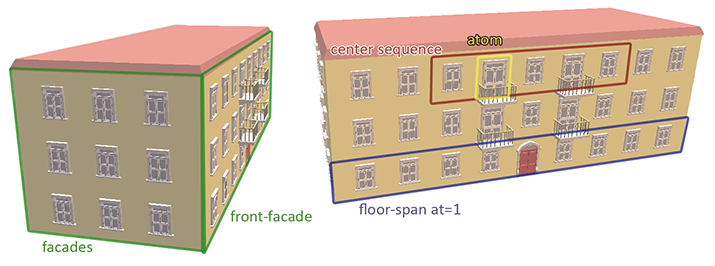
\includegraphics[width=\textwidth]{gfx/style.png}
	\caption{Resulting building of residential style. Several components are highlighted for comprehension.}
	\label{fig:style}
\end{figure}


\subsection{Building Instancing}


Once the building parameters have been gathered by the interface, the building needs to be generated.
Section \ref{design:building} Instancing a Building describes the procedure along with Figure \ref{fig:building}.
First the stroke is projected onto the construction plane and parsed by the shape recognizer as a rectangle.
The recognized rectangle dimensions serve as the blueprint which is extruded upwards for the measured height.
Then the building facades are generated according to the chosen style grammar and so is the ceiling.
The style grammar is fed each facade's dimensions and returns a set of spacings and facade elements that must be instanced
according to the rules defined in the style (see Fig.\ref{fig:style}).
To minimize the facade attachments in memory, a map of loaded attachments is managed so only the first instance of any
attachment is loaded.
Appendix \ref{residentialGrammar} lists the residential style depicted above.



\section{Content Editing}

All shapes in the system are made of 4-edged faces and all shapes are closed surfaces.
Operations such as the split by face loop rely on these properties.
Each shape computes each edge's neighboring faces (always 2)
and therefore each face's neighboring faces, forming an auxiliary structure called the edge map,
used for optimized queries for neighbors.

\subsection{Face Selection}

When a stroke finishes its start and ending points are projected onto the scene's available geometry.
If these 2 points lie on the same face of the same object that face is selected and the face contextual menu appears
(see Fig.\ref{fig:face-edge-selection-imp} bottom).

\begin{figure}[ht]
	\centering
		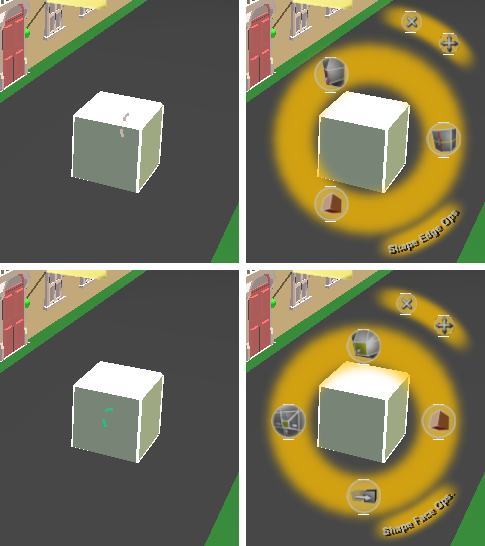
\includegraphics[scale=0.5]{gfx/face-edge-selection-imp.png}
	\caption{Edge and Face selection and their contextual menus}
	\label{fig:face-edge-selection-imp}
\end{figure}



\subsection{Edge Selection}

If the stroke start and ending points lie on different but neighboring faces of the same shape, the edge between
those faces is selected and the edge contextual menu appears
(see Fig.\ref{fig:face-edge-selection-imp} top).


\subsection{Determining and Selecting Directions}
\label{DIRECTIONS-LABEL}

In order to keep the interface simple and to minimize the number of steps needed to perform an operation,
a set of directions is estimated for edge and face selections
-- these are believed to be the most frequently needed vectors for shape operations.
When an edge is selected the computed directions are the edge outwards normal and the directions from the edge along its neighboring faces.
When a face is selected the computed directions are the face normal along with the 4 directions from the center of the face
to each of its neighboring faces (see Fig.\ref{fig:face-dirs}).

If an operation requires the user to select a direction from the user the computed directions are displayed centered on the selected aspect
and color coded. The interface relies on the user to keep drawing the stroke after the operation is triggered so the remaining of the stroke data parameterizes the operation.

\begin{figure}[ht]
	\centering
		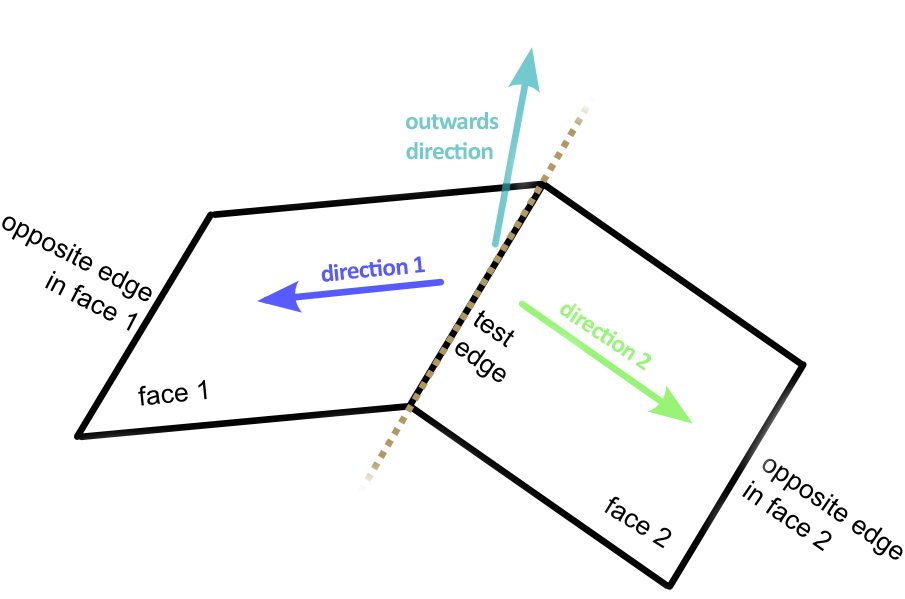
\includegraphics[scale=0.6]{gfx/face-dirs.png}
	\caption{Face directions}
	\label{fig:face-dirs}
\end{figure}


%\begin{figure}[ht]
%	\centering
%		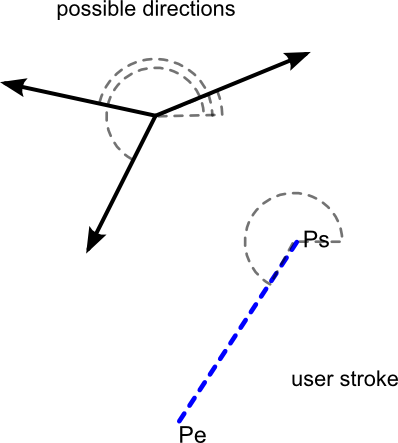
\includegraphics[scale=0.6]{gfx/election.png}
%	\caption{Direction selection}
%	\label{fig:election}
%\end{figure}




\subsection{Shape Operations}


This system has the goal of offering an easy yet reasonably powerful interface for modeling shapes.
The shape's internal structure was planned so both face and edge-based operations could be performed.
Every operation takes the triggering element (edge or face) as input parameter.
Most operations require additional information, obtained by extracting the user's stroke direction and length.
This interaction model keeps the number of stroke steps minimal while offering valid functionality for each operation.

The list of supported operations appears next, with them grouped by functional element -- the whole object, one of its
faces or one of its edges. Figure \ref{fig:ops} illustrates the application of these operations.

\begin{figure}[ht]
	\centering
		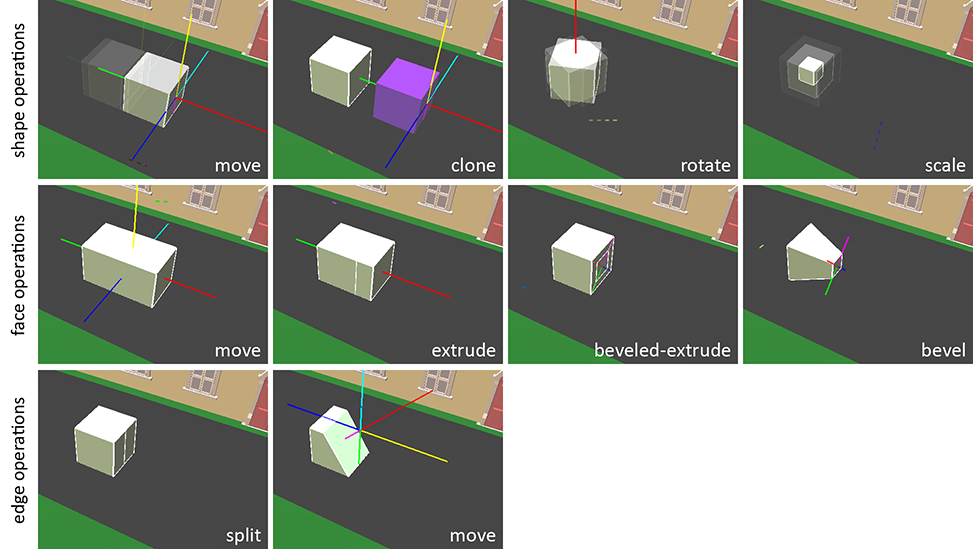
\includegraphics[width=\textwidth]{gfx/ops.png}
	\caption{Shape operation example applications}
	\label{fig:ops}
\end{figure}


\subsubsection{Object Operations}

Available object operations are \textbf{translation}, \textbf{rotation}, \textbf{scale} and \textbf{clone}.
The \textbf{translation} operation accepts a delta vector, applying it in real-time on one of the 5 directions:
normal and the 4 surrounding edge directions.
\textbf{Rotation} and \textbf{scale} operations take only the stroke length --
scale transforms all 3 axes proportionally;
rotation can take the triggered face's normal as axis of rotation or can default to the YY axis for simplification,
since most urban changing operations make use of this rotation.
An additional object operation is \textbf{cloning}. The clone operation works like a regular translation,
leaving behind a copy of the original shape.
Since it uses the face normal and face-bounding edges' directions, the cloning operation allows efficient generation
of building blocks and repetitive structures.


\subsubsection{Face Operations}

The \textbf{move} operation uses the same directions as translation, changing the position of the face vertices.
\textbf{Move neighbors} identifies neighboring faces having a smaller angle with the selected face than a defined threshold,
applying a move operation to the set of affected faces.
\textbf{Extrude} generates a new face for every face's edge and offers only the normal direction for moving the face outwards/inwards.
\textbf{Bevel} scales the face vertices, preserving inner angles.
The \textbf{beveled extrude} operation exists solely for convenience, generating a set of faces and applying an immediate bevel operation
to provide a simple way of creating relief details on faces for chimneys or windows.


\subsubsection{Edge Operations}

Edges can be \textbf{moved}, with the offered directions being the edge normal and the opposite edges along the neighboring faces.
This is illustrated on Figure \ref{fig:face-dirs} and described on section \ref{DIRECTIONS-LABEL}.

The \textbf{split along face loop} operation allows increasing the detail of a shape by cutting new faces along the center of the
implied edges.
\TODO{SPLIT}

On both edge and face context menus there's an option to \textbf{toggle} the visibility of the \textbf{shape edges}.


\subsubsection{Possible Additions}

The set of given operations offers a competent tool set for modeling simple shapes.
During tests users have found several creative ways of modeling the requested shapes.
Even so, multi-selection operations would be a nice addition to the tool set.
In early prototypes of the system the closed lasso stroke was used to select multiple objects, which proved problematic
since users inadvertently selected too many objects.
Furthermore, using multi-selection for shape operations limited the direction seeking algorithms described above,
which are key to the proposed simplified interface.



%By selecting a face the following operations can be performed (example applications on Fig.\ref{fig:ops}):
%\begin{itemize}
%	\item \textbf{extrude face} - Extrude generates 4 additional faces, getting the direction from the selected face's normal and the displacement from stroke length.
%	\item	\textbf{bevel face} - Bevel moves the face vertices, getting distance from stroke length.
%	\item	\textbf{extrude \& bevel} - This is a compound operation of zero length extrude followed by bevel. It exists for convenience to aid in the creation of holes for features such as windows or chimneys.
%	\item	\textbf{move face} - Move face displaces the face vertices, getting the direction from the selected face's normal and 4 computed directions.
%	\item	\textbf{move coplanar faces} - This operation works as the previous one but the neighboring faces having an angle with the selected one smaller than the threshold are also affected by the movement.
%\end{itemize}
%
%By selecting an edge the following operations can be performed:
%\begin{itemize}
%	\item \textbf{move edge} - Moves the edge vertices along one of the directions: edge normal and neighboring faces, obtaining the displacement from stroke length.
%	\item	\textbf{split at face loop} - The crossed edge defines a direction. All faces on that face loop are split in the middle, creating additional geometry. This operation has instant application as it doesn't require additional data.
%\end{itemize}
%
%On both edge and face context menus there's an option to \textbf{toggle} the visibility of the \textbf{shape edges}.
%
%All shapes have a stack of memento objects for supporting the undo operation, also available on both menus.
%The memento design pattern states that an auxiliary object - the memento object - decorates the state of the key object structures so they
%can be restored if backup is needed.


\section{Reviewing}

Notes can be created on the scene. A menu exists featuring a large area at the center where strokes can be drawn as if writing on paper.
A rubber option allows wiping the note contents. Once the note is written it can be attached to any scene object by using the
apply-to-scene concept (see Fig.\ref{fig:note}).
Notes are real 3D entities and can be hidden or edited by performing a closed stroke around them.

\begin{figure}[ht]
	\centering
		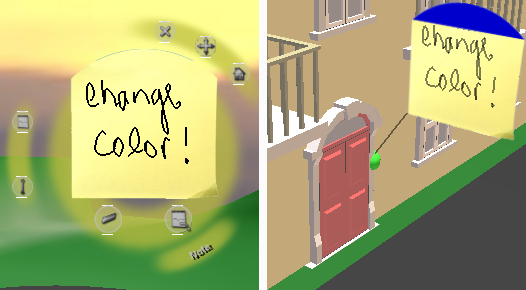
\includegraphics[scale=0.5]{gfx/note.png}
	\caption{Creating a note and the result attached to a door}
	\label{fig:note}
\end{figure}


\section{Proposed Work Flow}

Shapes can be loaded or saved to XML and the simple descriptive format can be easily supported by 3D modelers.
For the purposes of the generation of terrains, library objects and facade attachments the Blender 3D modeling package
was used and an exporting plug-in developed.

\subsection{Scenario Creation}

The system is a prototype tool so not much emphasis was put into the importing of content.
Even so, different scenarios could be created.
The height data from a terrain patch can be represented by either:
\begin{itemize}
	\item an height map - a gray-scale matrix with highest values represented by brighter colors.
	\item a topographic map - a discrete set of contour lines uniting points with the same altitude.
\end{itemize}

With any of these data a 3D mesh can be generated - by vertex shifting a regular mesh for height maps or applying
a Delaunay triangulation to the contour lines.
With additional satellite imagery the terrain appearance could also be approximated by vertex coloring or texture projection application.


\subsection{Building Style Creation}

New attachment shapes could be created using Urban Sketcher itself or an auxiliary 3D modeler.
Creating a building style is a matter of editing the style grammar, defining ceiling type, colors, floor height and most of all
the layout for the building floors using existing and/or newly created attachments.


\TODO{UPDATED WORK FLOW DIAGRAM}

\TODO{example stages}

